\documentclass[12pt,hyperref,a4paper,UTF8]{ctexart}
\usepackage{HDUReport}
\usepackage{listings}
\usepackage{xcolor}
\usepackage{graphicx}
\usepackage{setspace}
\usepackage{float}
\setstretch{1.5} % 设置全局行距为1.5倍

\usepackage{enumitem} % 载入enumitem包以便自定义列表环境
\setlist[itemize]{itemsep=0pt, parsep=0pt} % 设置itemize环境的项目间距和段落间距

\setmainfont{Times New Roman} % 英文正文为Times New Roman


\usepackage{tikz}
\usetikzlibrary{shapes.geometric, arrows}
\usetikzlibrary{positioning, arrows.meta}
\usetikzlibrary{calc}
%封面页设置
{   
    %标题
    \title{ 
        \vspace{1cm}
        \heiti \Huge \textbf{《单片机原理及应用》作业报告} \par
        \vspace{1cm} 
        \heiti \Large {\underline{实验报告4第一部分:2024数码管显示}   } 
        \vspace{3cm}
    
    }

    \author{
        \vspace{0.5cm}
        \kaishu\Large 学院\ \dlmu[9cm]{卓越学院} \\ %学院
        \vspace{0.5cm}
        \kaishu\Large 学号\ \dlmu[9cm]{23040447} \\ %班级
        \vspace{0.5cm}
        \kaishu\Large 姓名\ \dlmu[9cm]{陈文轩} \qquad  \\ %学号
        \vspace{0.5cm}
        \kaishu\Large 专业\ \dlmu[9cm]{智能硬件与系统(电子信息工程)} \qquad \\ %姓名 
    }
        
    \date{\today} % 默认为今天的日期,可以注释掉不显示日期
}
%%------------------------document环境开始------------------------%%
\begin{document}

%%-----------------------封面--------------------%%
\cover
\thispagestyle{empty} % 首页不显示页码
%%------------------摘要-------------%%
%\newpage
%\begin{abstract}




%\end{abstract}

%\thispagestyle{empty} % 首页不显示页码

%%--------------------------目录页------------------------%%
% \newpage
% \tableofcontents
% \thispagestyle{empty} % 目录不显示页码

%%------------------------正文页从这里开始-------------------%
\newpage
\setcounter{page}{1} % 让页码从正文开始编号

%%可选择这里也放一个标题
%\begin{center}
%    \title{ \Huge \textbf{{标题}}}
%\end{center}


\textbf{原题目:在LED显示器上用动态扫描方式实现2024四位数字显示。}


\section{实验代码}

\begin{lstlisting}[language=C, caption={实验程序}]

#include <reg51.h>//单片机头文件
unsigned char code Tab[]={0xC0,0xF9,0xA4,0xB0,0x99,0x92,0x82,0xF8,0x80,0x90};//共阳数码管码段表
unsigned char Dat[]={2,0,2,4};//存放4位数字数组
    
int i ,t;//定义变量,作为循环,定时计数
unsigned char tmp;//定义片选变量

void Delay()//延时子程序,作为数码管显示延迟
{
    unsigned char i;
    for(i=0;i<250;i++);
}
    
void main()
{

    while(1)//无限循环
    {
        tmp=0x01;//片选初值
        for(i=0;i<4;i++)//循环4次
        {
            P2=tmp;//片选初值
            P0=Tab[Dat[i]];//输出某一位数字的码段值
            tmp=tmp<<1;//片选值左移一位
            Delay();//调用延时
        }
    }
}

\end{lstlisting}

\section{实验效果}

\begin{figure}[H] % [H] 表示强制当前位置插入
    \centering
    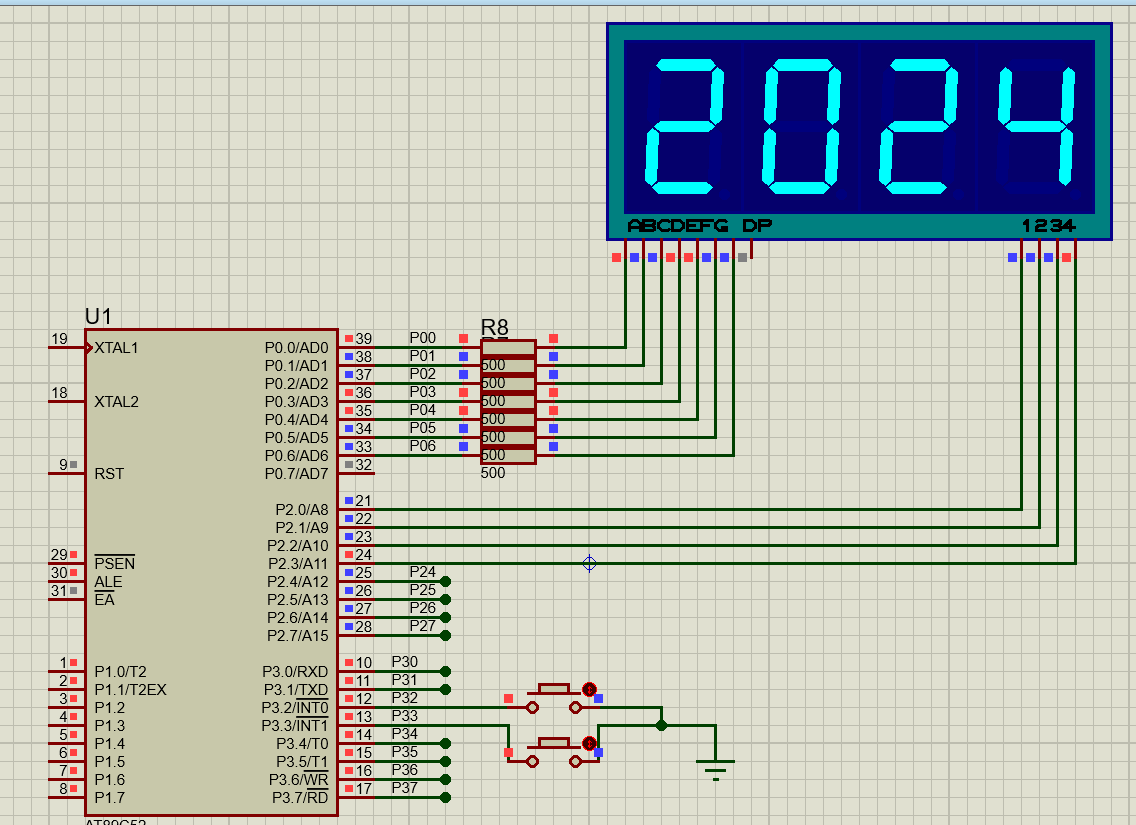
\includegraphics[width=0.9\textwidth]{figures/201.png} % 调整宽度为文本宽度的 80%
    \caption{2024显示效果 } %图片标题
    \label{fig:example} % 图片标签,用于引用
\end{figure}


\section{流程图}


\begin{figure}[H] % [H] 表示强制当前位置插入
        \centering
        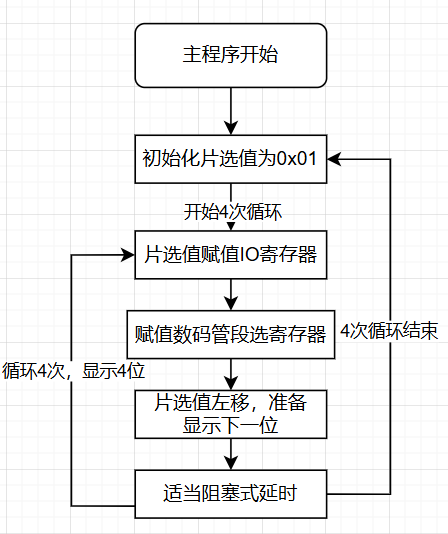
\includegraphics[width=0.9\textwidth]{figures/301.png} % 调整宽度为文本宽度的 80%
        \caption{系统控制流程图} %图片标题
        \label{fig:example} % 图片标签,用于引用
\end{figure}



\section{实验体会}


本实验通过动态扫描方式实现了数码管显示“2024”的功能,进一步掌握了单片机端口控制和数码管显示原理。实验中利用片选和段选实现了多位数码管的动态显示,延时函数确保了显示的稳定性。通过调试代码,初步理解了数码管码段表的作用及数据传输的时序要求。



\end{document}